\chapter{Operation}
\label{chap:Operation}

For the INSPIRE Mission Phase 0 study five basic mission phases have been defined. Nominal mission will last 30 earth days which is equal to 8.47 European days (MISSING REFERENCE). Furthermore a sixth optional mission phase after the nominal mission lifetime has been established which will be conducted if the rover is still operational after its nominal lifetime.

\begin{itemize}
\itemsep0pt
\item	\textbf{Phase 0:} Launch and Flight Phase
\item	\textbf{Phase 1:} Entry, Descent and Landing Phase
\item	\textbf{Phase 2:} Deployment Phase
\item	\textbf{Phase 3:} Egress, Commissioning and Early Operation Phase
\item	\textbf{Phase 4:} Mission Operation Phase
\item	(\textbf{Phase 5:} Exceeding Mission Operation Phase) 
\end{itemize}

\begin{figure}[H]
{\centering
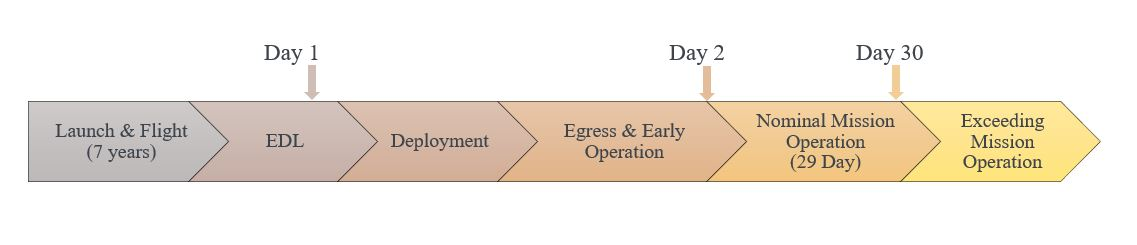
\includegraphics[width=1.0\textwidth]{Media/timeline}
\caption{Preliminary Mission Timeline for INSPIRE.}
\label{fig:timeline}
}
\end{figure}

Based on these missions phases some preliminary rover system modes as well as a basic mission timeline were concluded.

\section{Scientific Output}
\label{chap:sc-output}

Optical reference systems for path planning limit operation of the rover to an average of 41 h of sunlight out of 85 h in a European day \cite{Europa}. \autoref{fig:timeline-day} depicts a breakdown of possible continuous execution times in a mission day based on the power budget. Of course, the given order can be changed and, execution times can be adapted to fit the mission needs. \\

\begin{figure}[htb]
  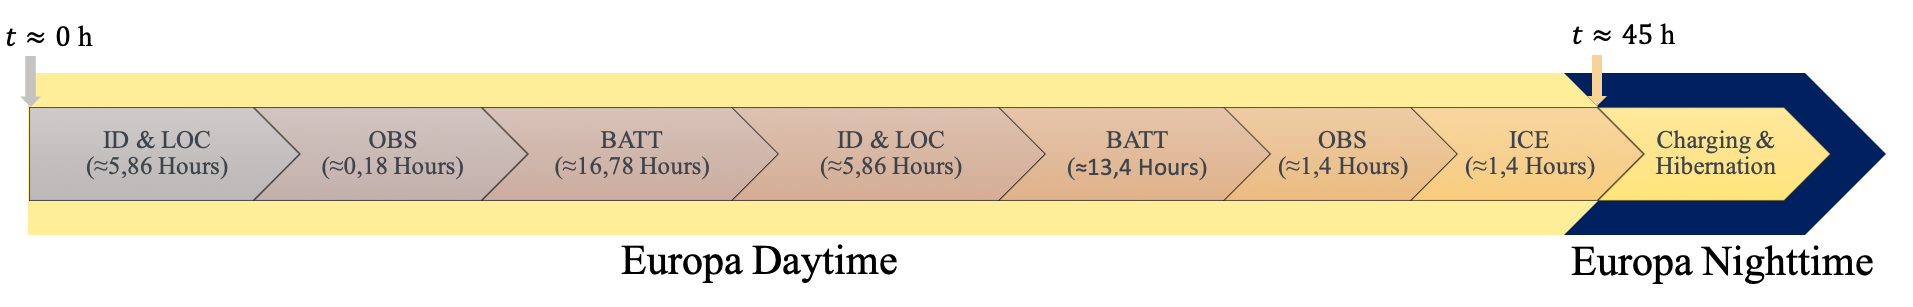
\includegraphics[width=1.0\textwidth]{Media/Timeline_day.png}
  \caption{Timeline of a mission day during phase 4}
  \label{fig:timeline-day}
\end{figure}


Locomotion phases consist of a sequence of mobility packages (MP). Each MP is built up of 5~min path planning and 10~s driving. Path planning time is estimated based on the limited processor speed (see \autoref{C&DH}). \\
Within the 6~h of a single Locomotion phase, a distance of 68~m is covered, resulting in a maximum distance of 1.7~km for the nominal mission.  \\

With respect to the payloads of the INSPIRE mission described in \autoref{chap:payload} the scientific return for phase 4 will consist of the data in \autoref{tab:SciDataOut}. Out of the 9~h of payload operation, a total of 6~h is used for imaging and radar measurements. \\
The total data output can be increased further in the case of a sufficient power margin during operation.

\begin{table}[h]
\centering
\caption{Expected scientific data output of the INSPIRE mission }
\begin{tabular}{lll}
\toprule
Payload         & Data Output                               & Data Output     \\ 
\midrule
GPR             & raw radar measurements                    & 40              \\
Cameras         & grayscale images with optional 3D mapping & >3570 images     \\
Sample Analyser & raw mineral analysis of ice core          & 10 - 12 samples \\
Solar Cells     & performance data                          & continuous      \\ 
\bottomrule
\end{tabular}
\label{tab:SciDataOut}
\end{table}

  
\section{Rover System Modes}
\label{chap:rovsubmod}
For this case study several rover system modes were defined. All ten modes are listed in \autoref{tab:systemmod}. 

They are separated into two groups. The design critical modes are displayed in white and are defined as system modes, which significantly influence the preliminary design of the rover subsystem like the thermal or power subsystem. None design critical modes (grey) also have a major influence on multiple subsystems of the rover but play a secondary role in the thermal and power budget of the rover for this Phase 0 study. These non design critical modes extend from the rover storage and launch until the finale deployment of the rover is completed. These modes and their design options depend heavily on the final design of the lander with which INSPIRE flies to Europe. Therefore, a clear definition of such modes is not possible at this time in the course of this phase 0 study. However, the respective considerations, preferences and options have been briefly described in the mode descriptions. It is important to note that INSPIRE's goal is to provide a flexible rover design with as few hard requirements as possible for the parent lander. Therefore, many aspects of the rover, as well as the none design critical modes, will need to be further defined and elaborated in later phases of the project in close consultation with the customer. \\
For example, the exact interfaces between rover and lander should be defined in more detail. Depending on the subsequently chosen interfaces, many possibilities may arise in the corresponding rover system modes. With an appropriate interface, for example, the excess electrical and thermal energy of the RTG, which is already active during the flight, could be used to supply the lander system with heat and power. A corresponding interface could also enable the transmission of health checks from INSPIRE. \\
The deployment phase will strongly depend on the final design of the lander, INSPIRE's position within the lander and also the possibilities that the lander provides to INSPIRE.
Possible deployment strategies would be as follows:

\begin{itemize}
\itemsep0pt
\item	\textbf{Option 1:} If INSPIRE on ground level: Release from storage box through spring mechanism or actuators. Rover storage configuration allows rolling and possible motorised actuation
\item	\textbf{Option 2:} If INSPIRE is above ground level: Similar as Option 1 but an additional ramp and ramp deployment would be required.
\item	\textbf{Option 3:} INSPIRE will be deployed through the landers robotic arm if it is capable of lifting its mass.
\end{itemize}
